\chapter{Famous Networks}
\section*{LeNet-5}
\begin{figure}[h]
  \centering
  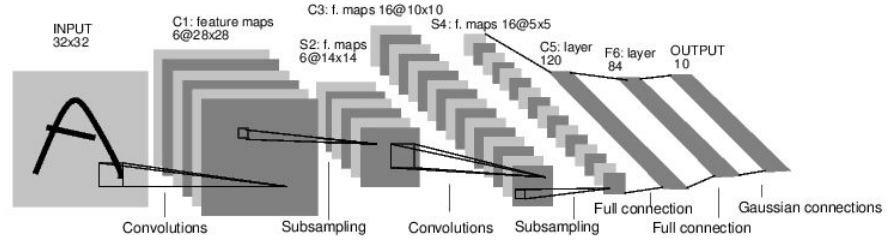
\includegraphics[width=0.8\textwidth]{Images/famous_networks/1.png}
  \caption{LeNet}
\end{figure}
The first successful applications of Convolutional Networks were developed by Yann LeCun in 1990’s. Of these, the best known is the LeNet architecture that was used to read zip codes, digits, etc.

\section*{AlexNet}
The first work that popularized Convolutional Networks in Computer Vision was the AlexNet, developed by Alex Krizhevsky, Ilya Sutskever and Geoff Hinton. The AlexNet was submitted to the ImageNet ILSVRC challenge in 2012 and significantly outperformed the second runner-up (top 5 error of 16\% compared to runner-up with 26\% error). The Network had a very similar architecture to LeNet, but was deeper, bigger, and featured Convolutional Layers stacked on top of each other (previously it was common to only have a single CONV layer always immediately followed by a POOL layer). 60M parameters.

\begin{figure}[h]
  \centering
  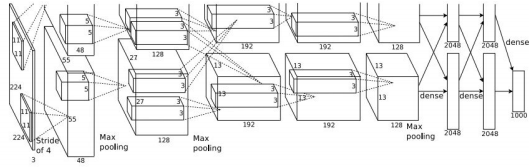
\includegraphics[width=0.8\textwidth]{Images/famous_networks/2.png}
  \caption{AlexNet. There is an error in the paper figure, the input image must be of 227 so that the rest of volumes are coherent}
\end{figure}

\section*{VGGNet}
The runner-up in ILSVRC 2014 was the network from Karen Simonyan and Andrew Zisserman that became known as the VGGNet. Its main contribution was in showing that the depth of the network is a critical component for good performance. Their final best network contains 16 CONV/FC layers and, appealingly, features an extremely homogeneous architecture that only performs $3 \times 3$ convolutions and $2 \times 2$ pooling from the beginning to the end. Their pretrained model is available for plug and play use in Caffe. A downside of the VGGNet is that it is more expensive to evaluate and uses a lot more memory and parameters (140M). Most of these parameters are in the first fully connected layer, and it was since found that these FC layers can be removed with no performance downgrade, significantly reducing the number of necessary parameters.

The most of the network parameters are in the FC layer and most of the memory required by the network is used in the first 2 ConvLayers.

\begin{figure}[h]
  \centering
  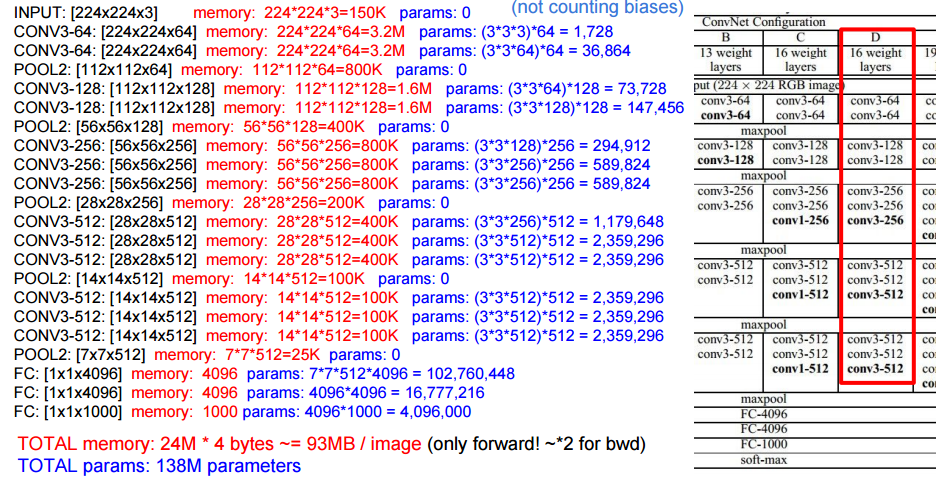
\includegraphics[width=0.8\textwidth]{Images/famous_networks/3.png}
  \caption{VGGNet - 7.3\% top 5 error in ImageNet}
\end{figure}

\section*{GoogLeNet}
The ILSVRC 2014 winner was a Convolutional Network from Szegedy et al. from Google. Its main contribution was the development of an Inception Module that dramatically reduced the number of parameters in the network (4M, compared to AlexNet with 60M). Additionally, this paper uses Average Pooling instead of Fully Connected layers at the top of the ConvNet, eliminating a large amount of parameters that do not seem to matter much. There are also several followup versions to the GoogLeNet, most recently Inception-v4. 
\begin{figure}[h]
  \centering
  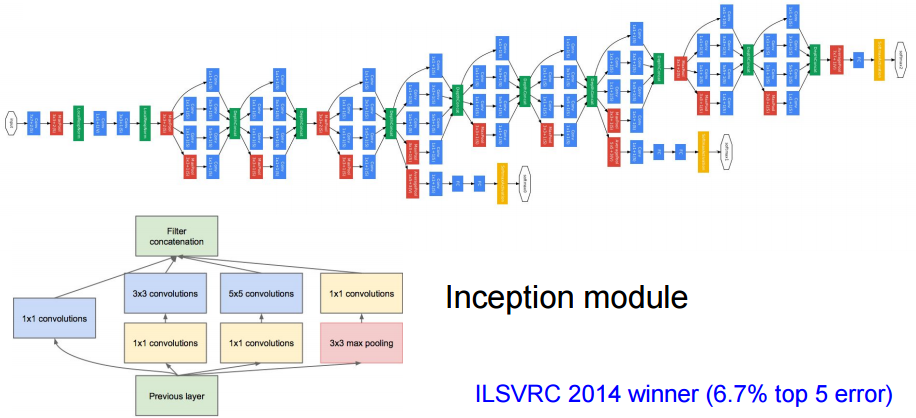
\includegraphics[width=0.8\textwidth]{Images/famous_networks/4.png}
  \caption{VGGNet - 6.7\% top 5 error in ImageNet}
\end{figure}
\begin{figure}[h]
  \centering
  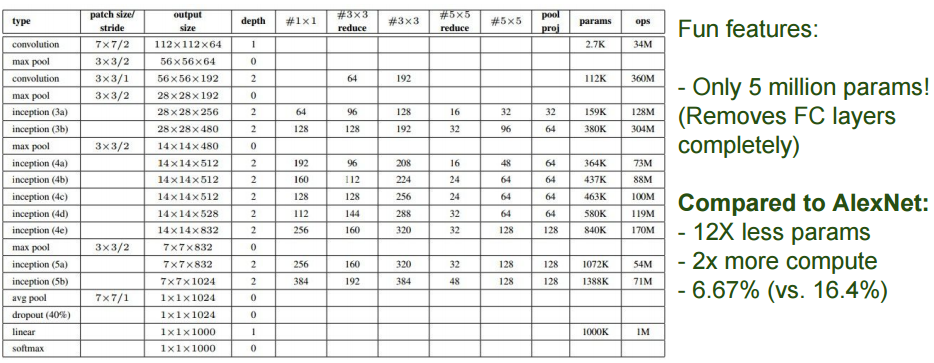
\includegraphics[width=0.8\textwidth]{Images/famous_networks/5.png}
  \caption{VGGNet structure}
\end{figure}

\section*{ResNet}
Let $H(x)$ be a function that you desire to obtian. In a typical net you would compute a squence of steps \texttt{ReLu(ReLu(xw1+b1)*w2+b2)} to transform $x$ to $H(x)$. Instead, in a ResNet you compute a delta to be added to the original input to obtain $H(x)$.

What is nice about it is that in \textit{plain nets}, gradients must flow through all the transformations. Instead, in \textit{residual nets} because it is addition (distributes the gradient equally to all its children), the gradient with flow through the (weights, ReLU) but will also skip this transformations and will go directly to the previous part and flow directly to the previous block. So the gradients can skip all the transformations and go directly to the first layer. In this way, you can train very fast the first layer which is doing simple statistics, and the rest of layers will learn to add to the single in between to make it work at the end.

\begin{figure}[h]
  \centering
  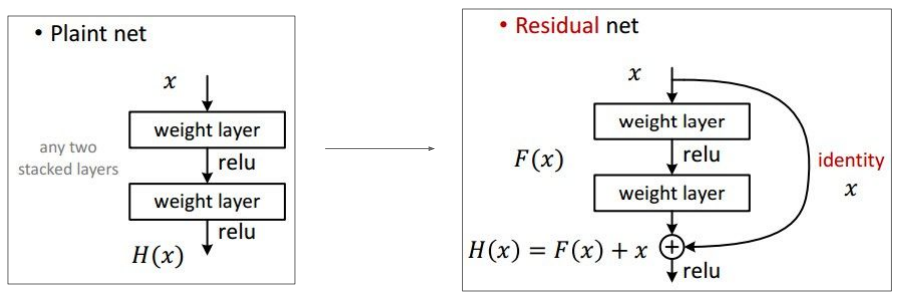
\includegraphics[width=0.6\textwidth]{Images/famous_networks/6.png}
  \caption{Plain vs Residual Net}
\end{figure}

\begin{figure}[h]
  \centering
  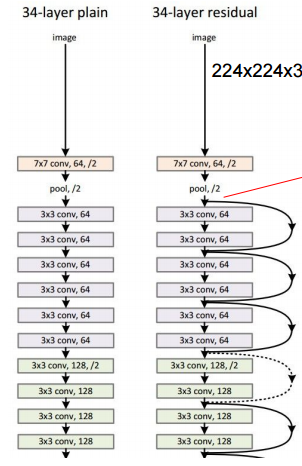
\includegraphics[width=0.3\textwidth]{Images/famous_networks/7.png}
  \caption{ResNet (much more layers than the ones on the diagram)}
\end{figure}

Another way of seeing it, it that ResNets are only computing a delta on top of the identity. So it makes it nice to optimize.

 Residual Network developed by Kaiming He et al. was the winner of ILSVRC 2015. It features specialskip connections and a heavy use of batch normalization. The architecture is also missing fully connected layers at the end of the network. ResNets are currently by far state of the art Convolutional Neural Network models and are the default choice for using ConvNets in practice (as of May 10, 2016). In particular, also see more recent developments that tweak the original architecture from Kaiming He et al. Identity Mappings in Deep Residual Networks (published March 2016).
It is interesting that after the first layer they do polling (the only polling in all the net) and they scale the input image of $244 \times 244$ to $56 \times 56$, and the net works that well. Its crazy that all the layer (except the first one) work wit $56 \times 56 \times ?$ and even compressing the data this much it has a high accuracy.


\begin{figure}[h]
  \centering
  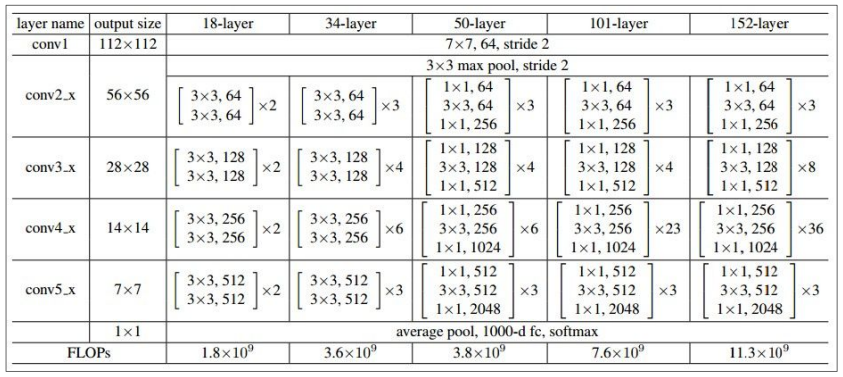
\includegraphics[width=0.8\textwidth]{Images/famous_networks/9.png}
  \caption{ResNet structure. 3.6\% top 5 error in ImageNet, 152 layers, 2-3 weeks training on 8 GPU machine, faster at test time that VGGNet}
\end{figure}

\section*{Should we add infinite layers?}
In plot \ref{fig:depth_rev} it is clear that networks are getting deeper and deeper
\begin{figure}[h]
  \centering
  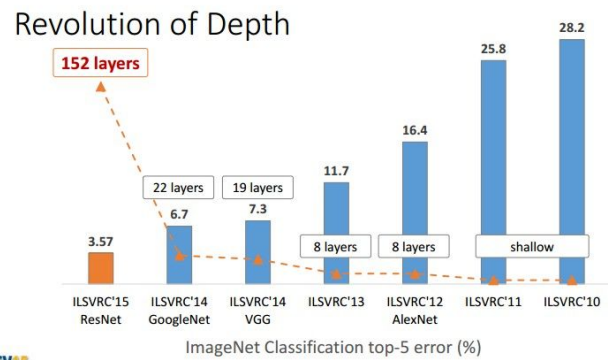
\includegraphics[width=0.4\textwidth]{Images/famous_networks/10.png}
  \caption{Depth revolution}
  \label{fig:depth_rev}
\end{figure}
But we have to be careful. Plot \ref{fig:cifar_train_error} shows CIFAR-10 training error. In the left plain nets (weighted layer + ReLU) in the right ResNet. How it is possible to get a higher training error (dashed lines) with higher number of layers? It should not happen, the model is more complex. The explanation is that we are still not capable of optimizing them good enough.

\begin{figure}[h]
  \centering
  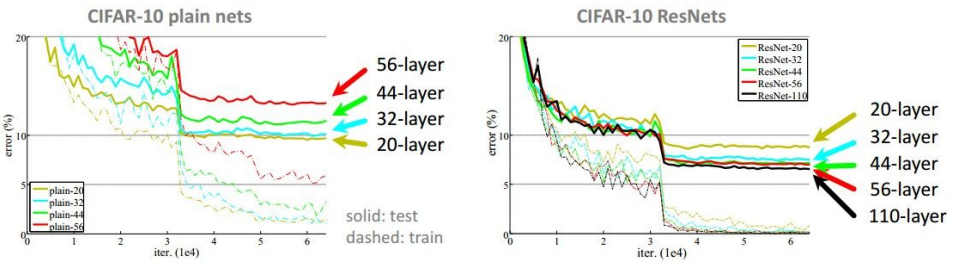
\includegraphics[width=0.8\textwidth]{Images/famous_networks/11.png}
  \caption{CIFAR-10 training error}
  \label{fig:cifar_train_error}
\end{figure}

However, ResNets always improve the test and training error.

So the answer to the question is that we should keep adding more layers but not in a naive way, we should do it in a ResNet way